\documentclass{article}
\title{Notes for: Generative Aversarial User Model for Reinforcement Learning Based Recommendation System}
\author{Michael Nefiodovas. \thanks{paper: https://arxiv.org/pdf/1812.10613.pdf}}
\date{\today}
\usepackage{graphicx}

\begin{document}
    \maketitle

    \section{Setting}

    \subsection{Intuition}
    \begin{itemize}
        \item You work at YouTube and want to recommend YouTube videos to your users to maximise their "utility" from watching videos.
        \item You have access to a set of all available videos (all YouTube videos) to show the user.
        \item You must design an algorithm to select a subset of videos to recommend to the user after they watch a video.
        \item Once shown a selection of recommendations, the user may click on one of the videos to watch or may abstain from clicking.
        \item You have access to users' historical view data.
        \item[Summary:] \emph{users are recommended a page of items and they provide feedback, and then the system recommends a new page of items.}
    \end{itemize}

    \subsection{Assumptions}
    \begin{enumerate}
        \item Users are not random and given a set of $k$ items, users will attempt to maximise their own reward/utility $r$.
        \item Watching each video incurs an opportunity cost, if watching a video is a waste of time or mental energy the user can choose to \emph{not} click on any recommendations.
        \item Reward is the marginal benefit of taking an action, this means that $r$ depends not only on the video about to be watched but also the user's watch history leading up to this video\footnote{Someone might not be interested in Taylor Swift at the beginning but do become interested after listening to it. Users may also get bored if they watch the same video 100 times}.
    \end{enumerate}

    \section{Framing}
    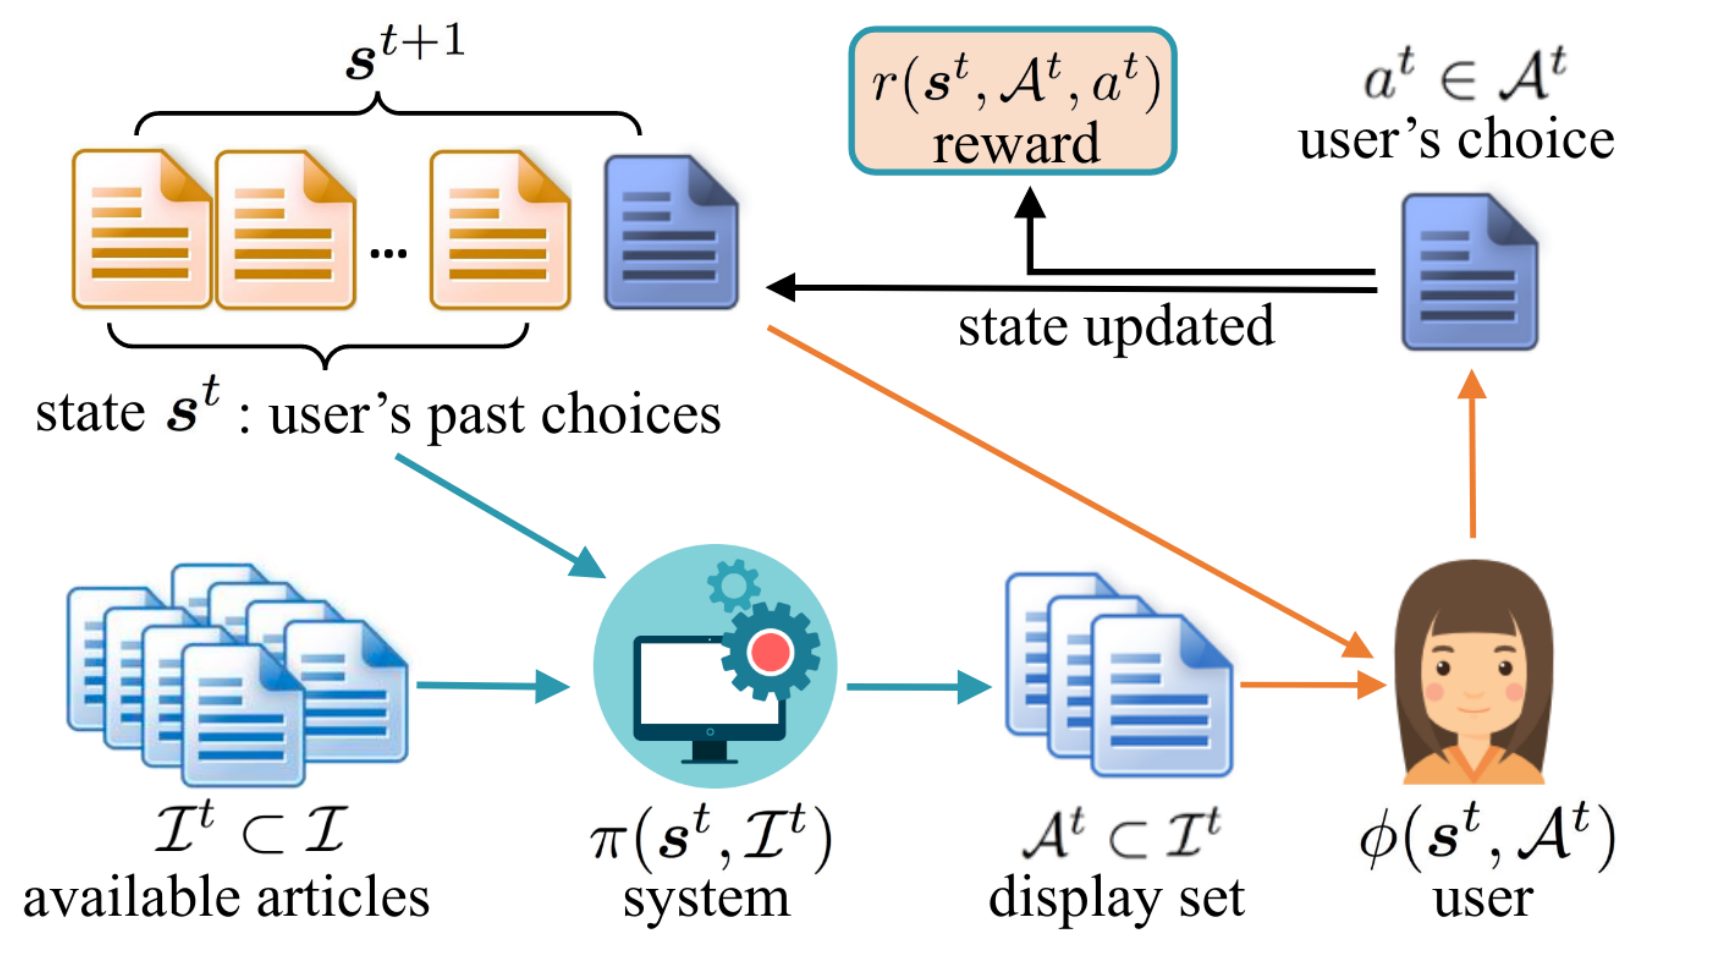
\includegraphics[width=10cm]{fig1.png}
    
    \textbf{Environment}

    It may be strange to think about it at first but:
    The "user" in this scenario is the environment which we interact with by selecting videos/documents to recommend. The user obeys their policy $\phi ^* (S^t, A^t)$, selecting a choice based on the current state and the recommending agent's selected action (what videos were shown).

    \textbf{State}

    The current environment state $s^t$ refers to "an ordered sequenceof a user’s historical clicks"

    \textbf{Action}

    The action is a selection of videos to present the user, that means if there is $\mathcal{I}$ total available videos to select from and you are showing the user $k$ ideos at a time, then action $A^t$ is selected $A^t \in {\mathcal{I^t} \choose k}$. As you can imagine, the possible action space is absolutely huge even for medium sized $I^t$ and $k$*. 

    *This problem is addressed through their \emph{Cascading Q-Network} architecture.

    \textbf{Reward}

    \section{Contribution}

    \subsection{Generative Adversarial User Model}


    \subsection{Cascading RL Policy for Recommendation}


\end{document}